%
% tikztemplate.tex -- Template für standalone TIKZ Bilder
%
% (c) 2019 Prof Dr Andreas Müller, Hochschule Rapperswil
%
\documentclass[tikz,12pt]{standalone}
\usepackage{amsmath}
\usepackage{times}
\usepackage{txfonts}
\usepackage{pgfplots}
\usepackage{csvsimple}
\usetikzlibrary{arrows,intersections,math}
\begin{document}
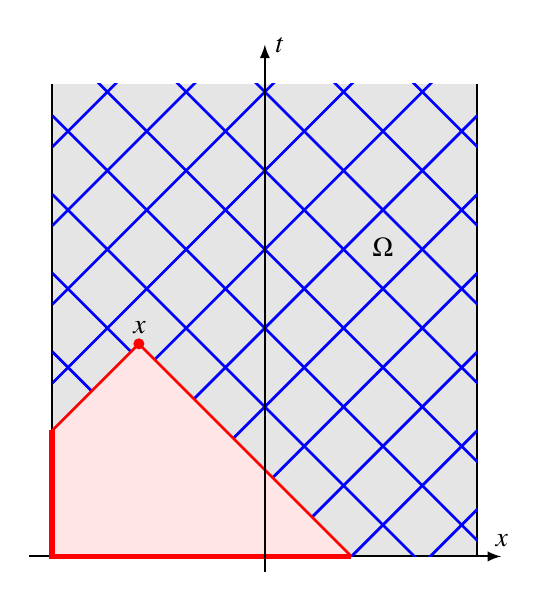
\begin{tikzpicture}[>=latex]

\def\radius{2.7}
\def\x{-1.6}
\def\y{2.7}

\coordinate (X) at (\x,\y);
\coordinate (A) at ({-\radius},{\y-(\x+\radius)});
\coordinate (B) at (-\radius,0);
\coordinate (C) at ({\x+\y},0);
\coordinate (D) at (\radius,0);

\fill[color=gray!20] (B)--(D)--(\radius,6)--(-\radius,6)--cycle;
\draw[line width=0.7pt] (B)--(-\radius,6);
\draw[line width=0.7pt] (D)--(\radius,6);
\draw[->,line width=0.7pt] (-3,0)--(3,0) coordinate[label={$x$}];

\begin{scope}
\clip (B) rectangle (\radius,6);
\foreach\cy in {-3.1,-2.1,...,9}{
	\draw[color=blue,line width=1pt]
		({-\radius},{\cy-\radius})--({\radius},{\cy+\radius});
	\draw[color=blue,line width=1pt]
		({-\radius},{\cy+\radius})--({\radius},{\cy-\radius});
}
\end{scope}

\fill[color=red!10] (X)--(A)--(B)--(C)--cycle;
\draw[color=red,line width=1pt] (X)--(A);
\draw[color=red,line width=1pt] (X)--(C);
\draw[color=red,line width=2pt] (A)--(B)--(C);

\draw[->,line width=0.7pt] (0,-0.2)--(0,6.5) coordinate[label={right:$t$}];

\node at (1.5,3.93) {$\Omega$};

\node at (X) [above] {$x$};
\fill[color=red] (X) circle[radius=2pt];

\end{tikzpicture}
\end{document}
